\chapter{The Compact Muon Solenoid Detector}
\label{chap:CMS}

The \ac{CMS} detector~\cite{CMS:2008xjf} is one of the two general-purpose detectors involved in the discovery of the Higgs boson in 2012~\cite{ATLAS:2012yve,CMS:2012qbp}. It is located around 100 meters underground near the French town of Cessy. The full detector weights over 14 thousand tones, and is roughly cylindrically symmetric with a length and diameter of 21 and 15 meters, respectively. It consists of several layers of subsystems, as illustrated in Figure~\ref{fig:CMS}.

\begin{figure}[tbh!]
 \begin{center}
 \begin{tabular}{c}
 \includegraphics[width=0.8\textwidth]{figures/Part2/CMS/cms}
 \end{tabular}
 \caption{A sectional view of the \ac{CMS} detector, adapted from~\cite{Sakuma:2013jqa}.}
 \label{fig:CMS}
 \end{center}
\end{figure}

Brief descriptions of these subsystems are given in \autoref{sec:TK}-\autoref{sec:TrigSys}. The coordinate system adopted by \ac{CMS} is introduced in \autoref{sec:Coord}.

\section{Coordinate System Used in the CMS Detector}
\label{sec:Coord}

As illustrated in Figure~\ref{fig:axis3D}, the coordinate system adopted by \ac{CMS} uses the nominal \ac{IP} as its origin, with the x-axis pointing radially inward towards the center of the \ac{LHC} ring, the y-axis pointing vertically upward towards the sky, and the z-axis pointing along the beam line towards west of the detector.

\begin{figure}[tbh!]
 \begin{center}
 \begin{tabular}{c}
 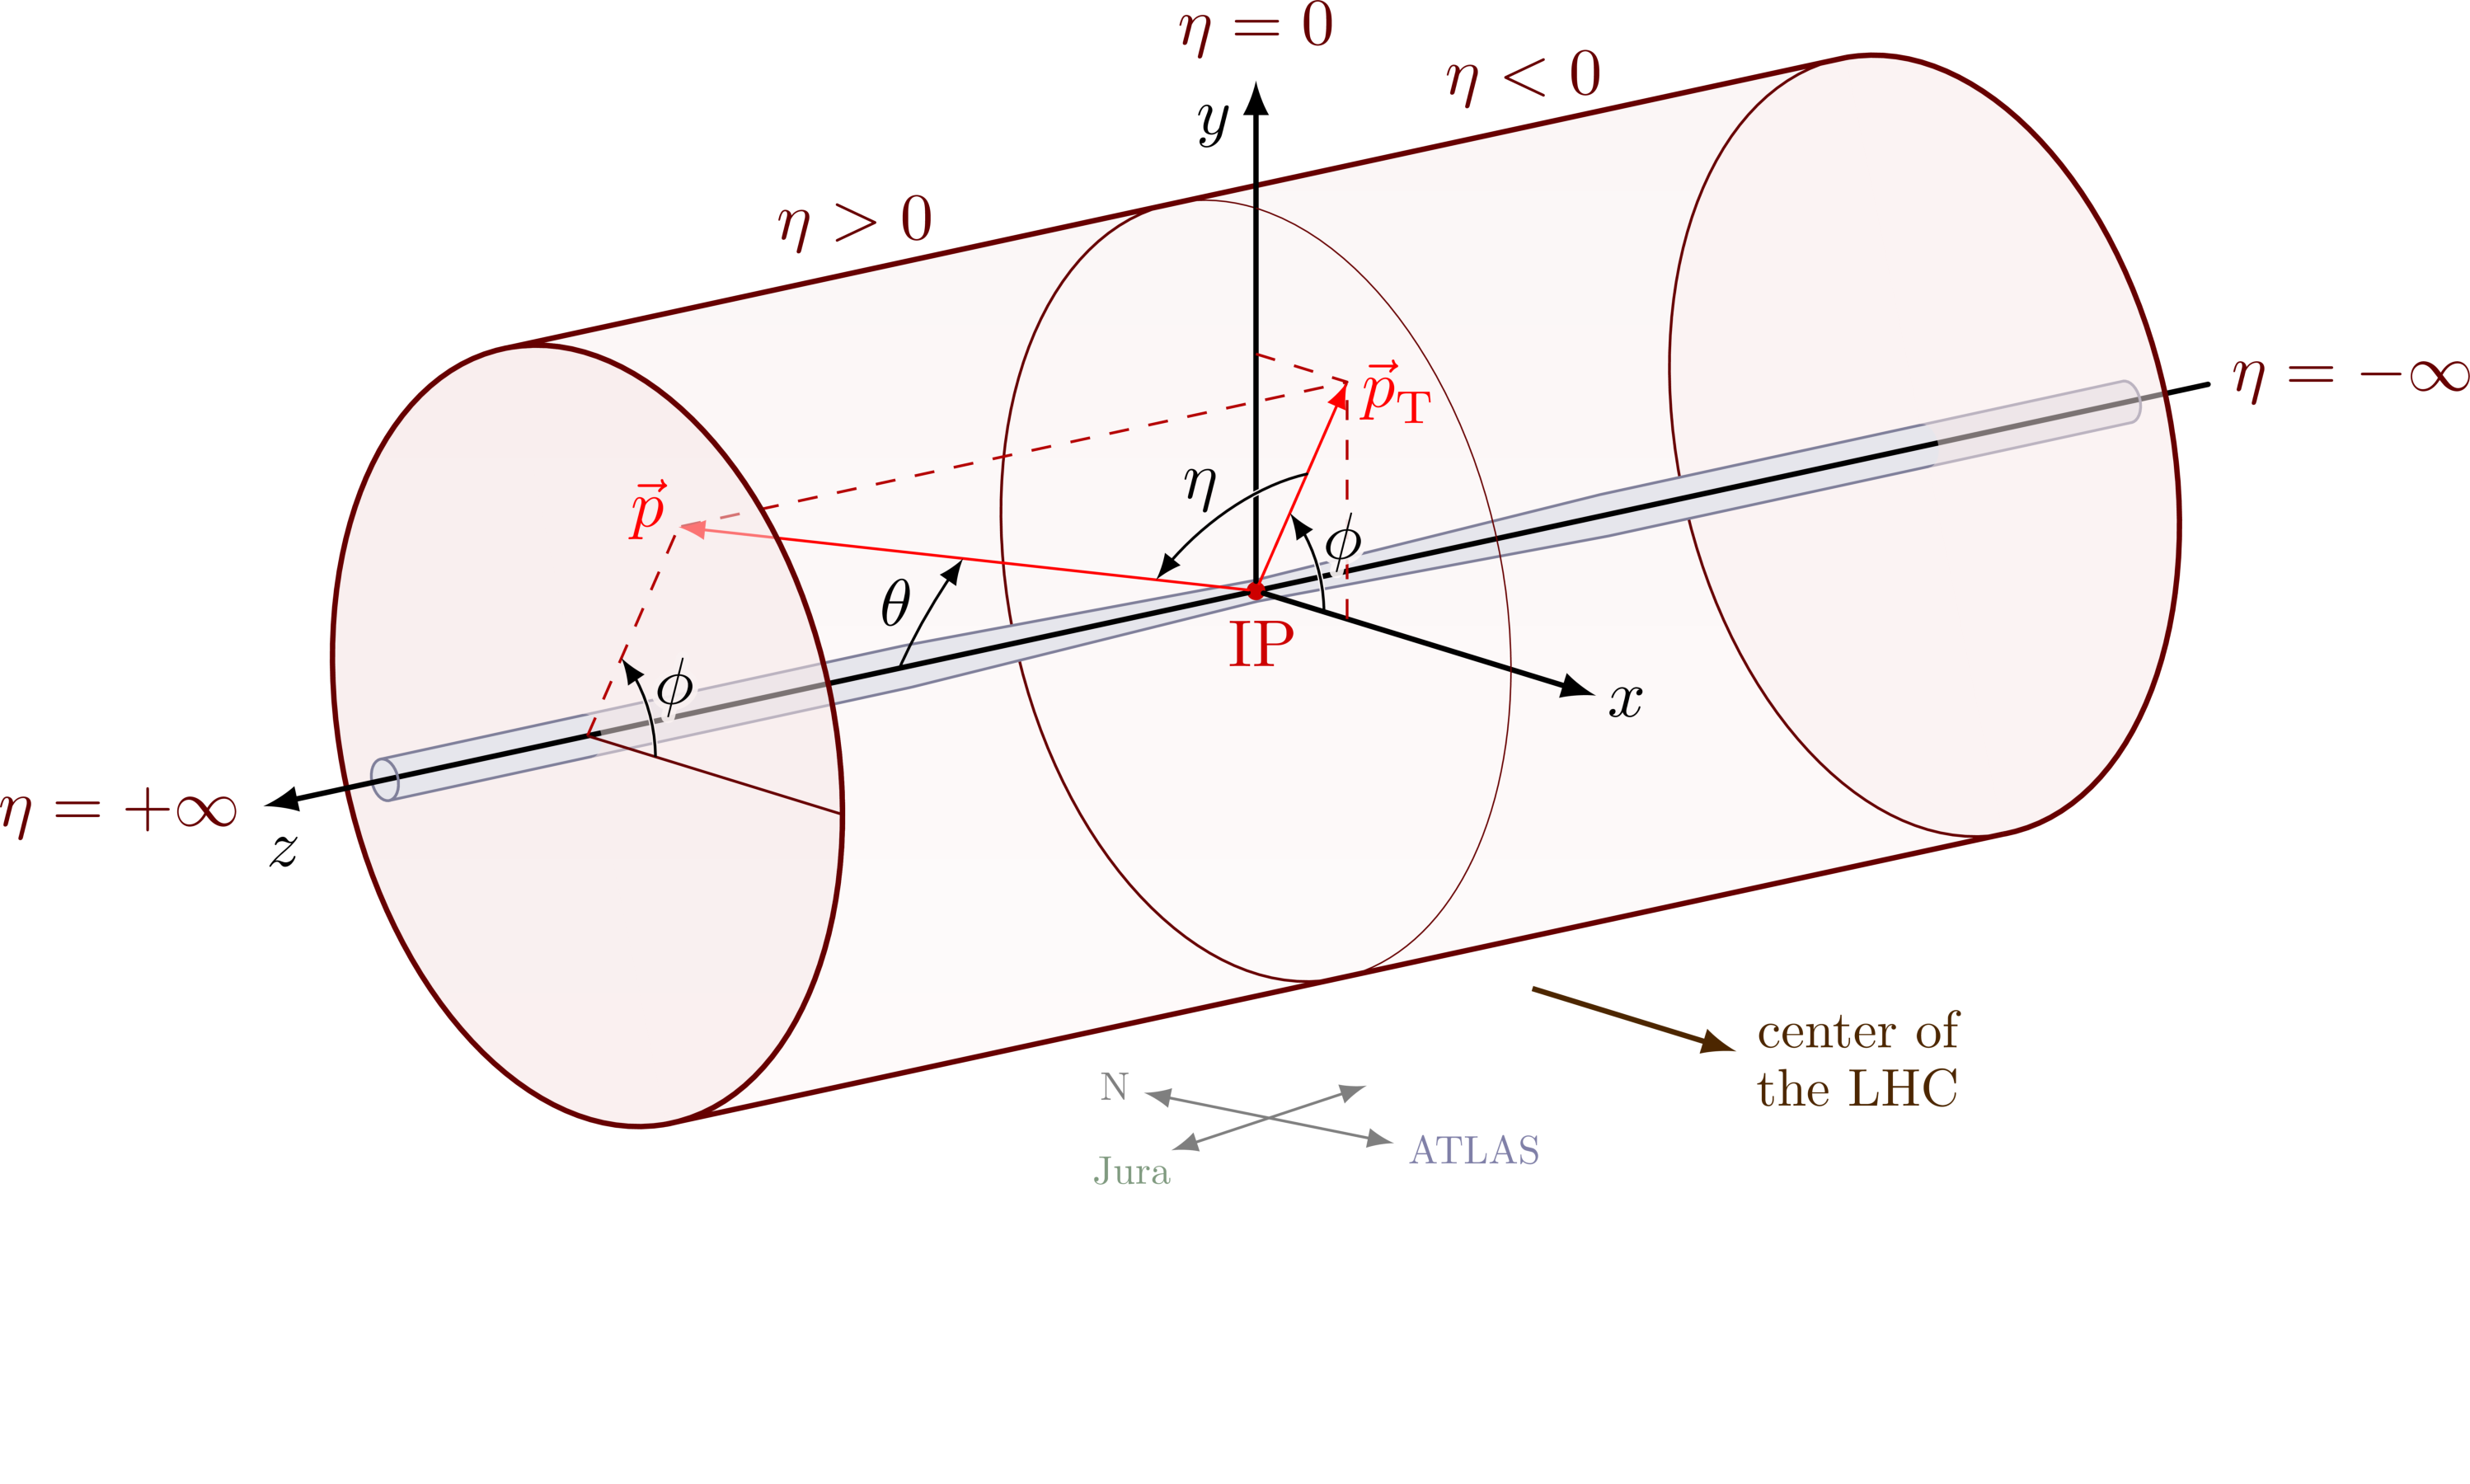
\includegraphics[width=0.8\textwidth]{figures/Part2/CMS/axis3D_CMS-004}
 \end{tabular}
 \caption{A sketch of the coordinate system adopted by \ac{CMS}, adapted from~\cite{tikz:3D}.}
 \label{fig:axis3D}
 \end{center}
\end{figure}

The x- and y-axis form the transverse plane as they are both orthogonal to the beam line (z-axis). The distance from the \ac{IP} in the transverse plane is defined as $r=\sqrt{x^2+y^2}$. Variables defined entirely in the transverse plane, such as $\pt$, \MET, and $\Ht$, are often indicated by a subscripted T. The azimuthal angle $\phi$ is measured from the positive x-axis and the polar angle $\theta$ is measured from the positive z-axis. Another variable $\eta$, known as pseudorapidity, is defined as

\begin{equation}
\eta=-\ln(\frac{\theta}{2}).
\end{equation}

It is preferred over $\theta$ mainly due to: i) particle production rate is roughly uniform in this variable, and ii) a difference in this variables, denoted by $\mathrm{\Delta}\eta$, is invariant under Lorentz boosts. The conversion between $\eta$ and $\theta$ is illustrated in Figure~\ref{fig:axis2D}. The $\mathrm{\Delta}\eta$ and the difference in azimuthal angles, denoted by $\mathrm{\Delta}\phi$, are used to define the distance parameter $\mathrm{\Delta}R$

\begin{equation}
\label{eq:DR}
\mathrm{\Delta}R=\sqrt{\mathrm{\Delta}\eta^2+\mathrm{\Delta}\phi^2}.
\end{equation}

\begin{figure}[tbh!]
 \begin{center}
 \begin{tabular}{c}
 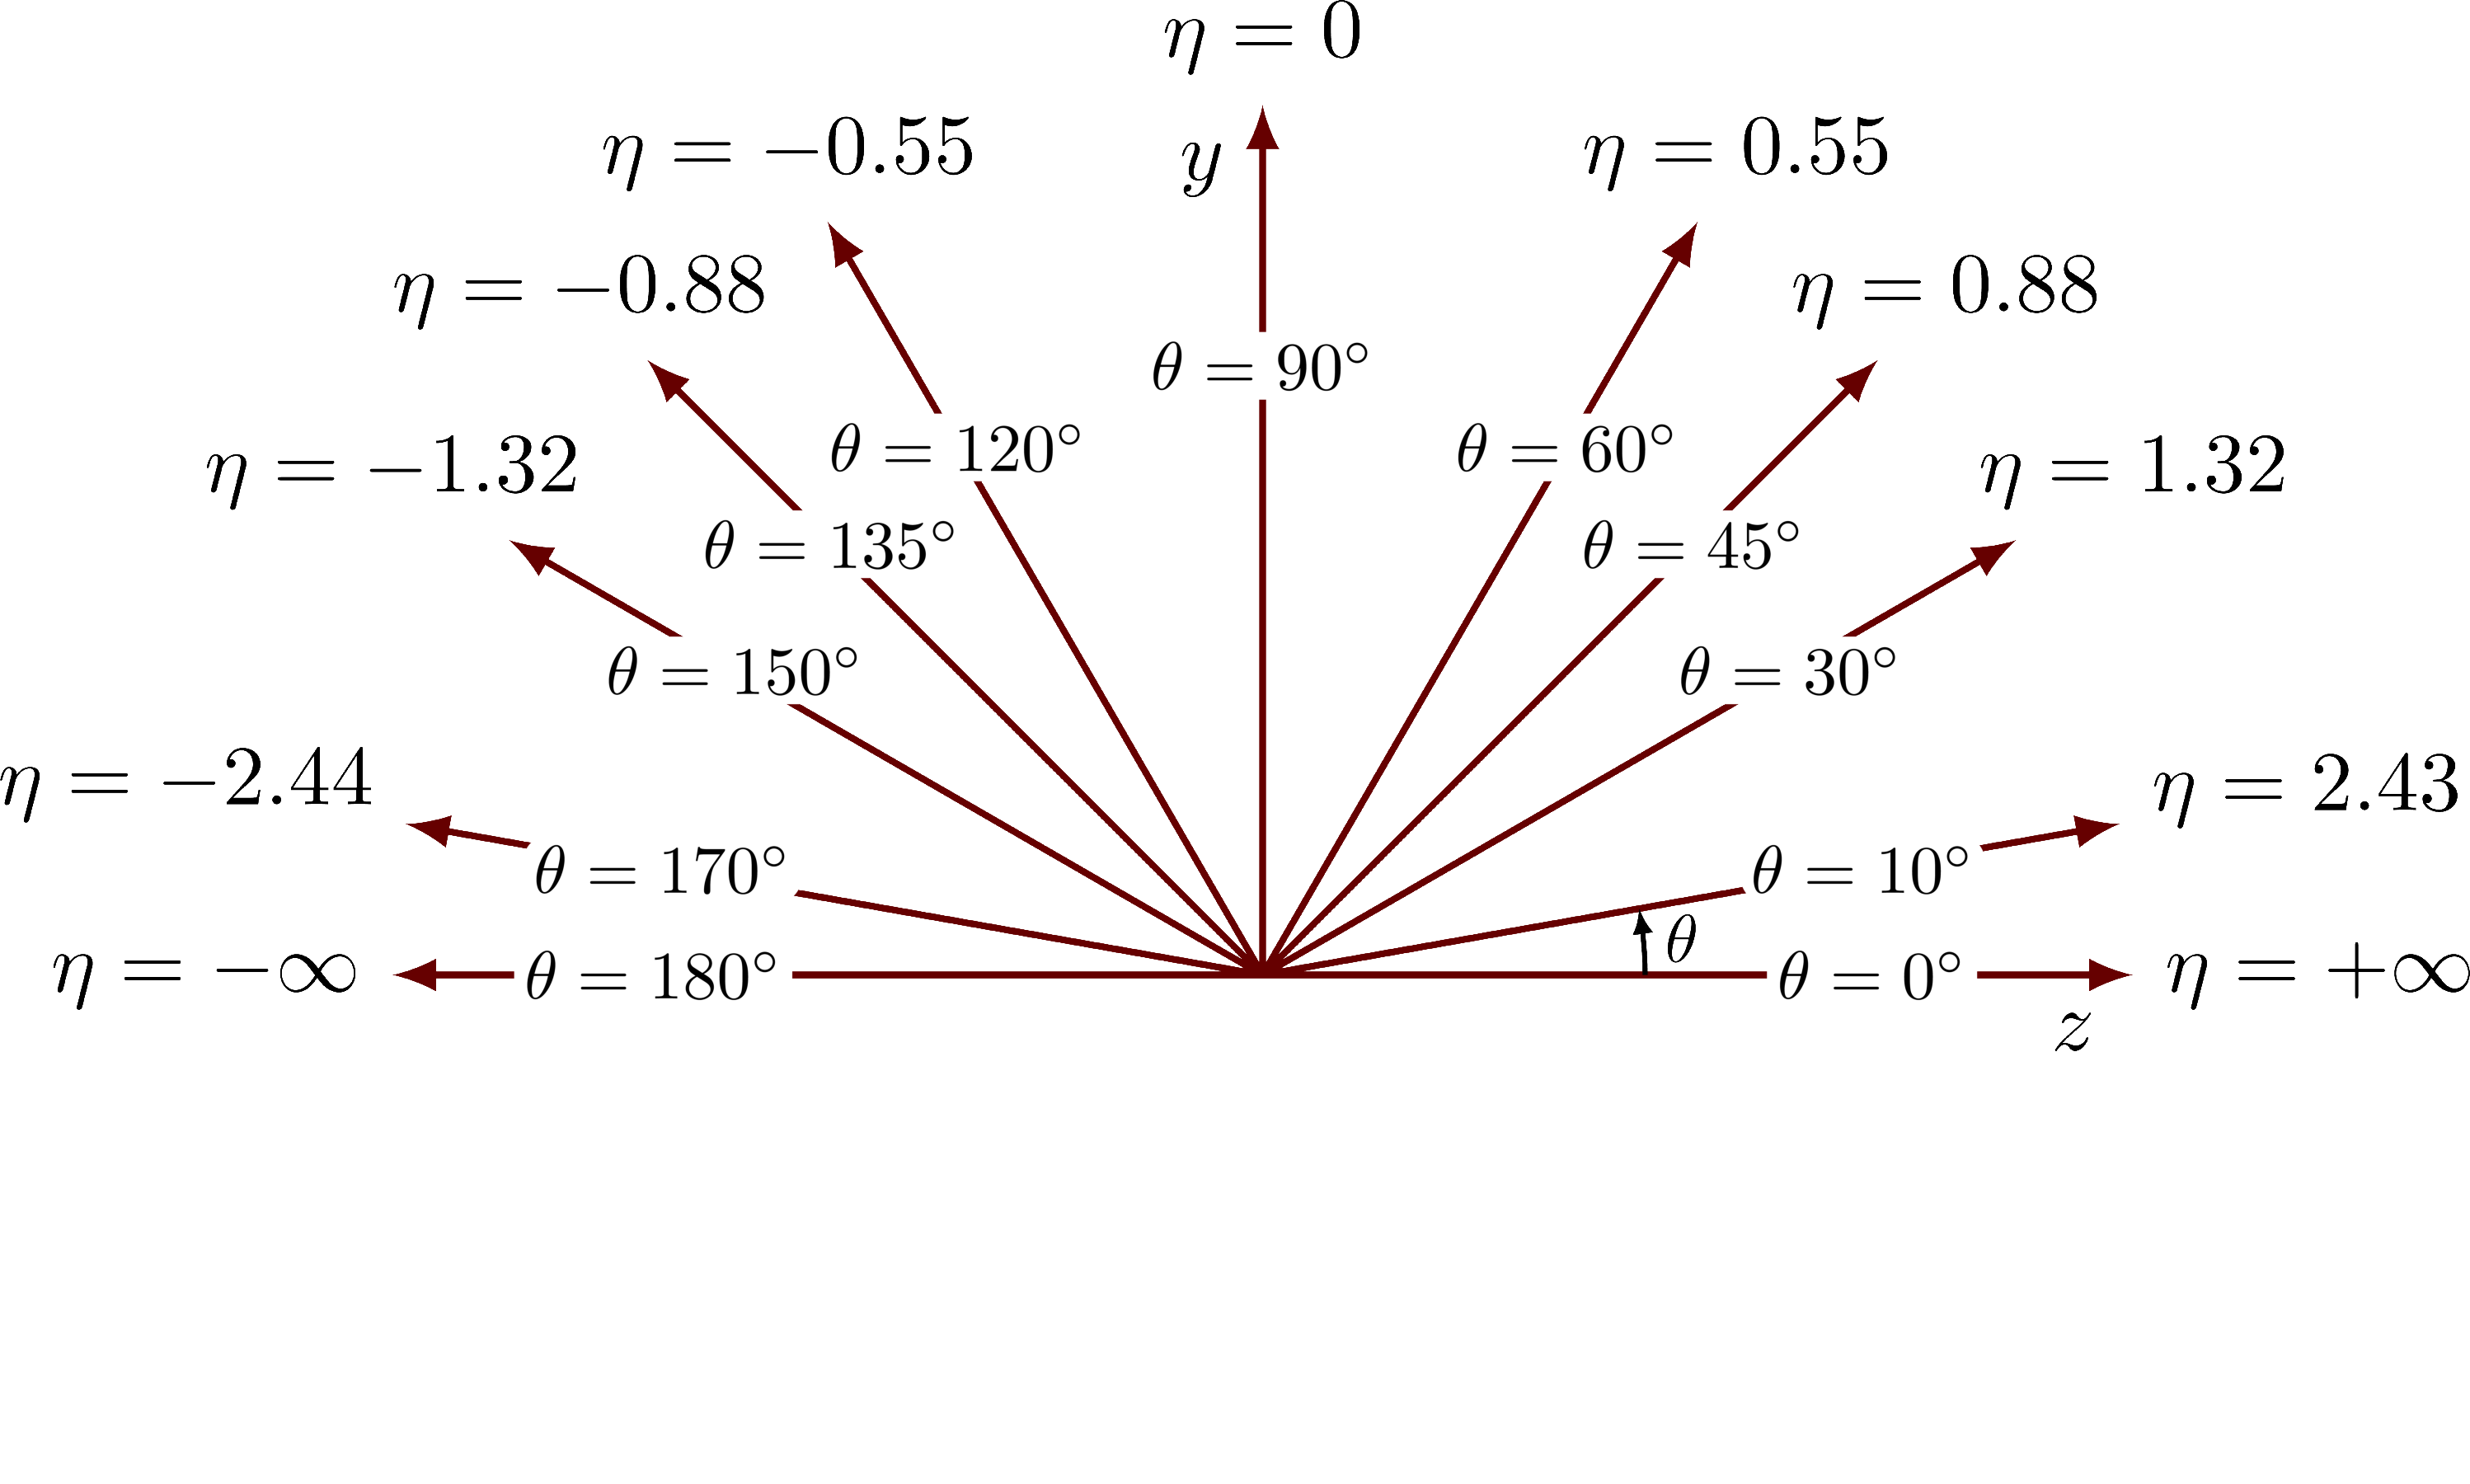
\includegraphics[width=0.8\textwidth]{figures/Part2/CMS/axis2D_pseudorapidity-003}
 \end{tabular}
 \caption{Examples of the conversion between the polar angle $\theta$ and the pseudorapidity $\eta$, adapted from~\cite{tikz:2D}.}
 \label{fig:axis2D}
 \end{center}
\end{figure}

\section{The Tracking System}
\label{sec:TK}

The tracking system is the innermost subsystem of the \ac{CMS} detector where the density of particles from the collisions is the highest. 

\begin{figure}[tbh!]
 \begin{center}
 \begin{tabular}{c}
 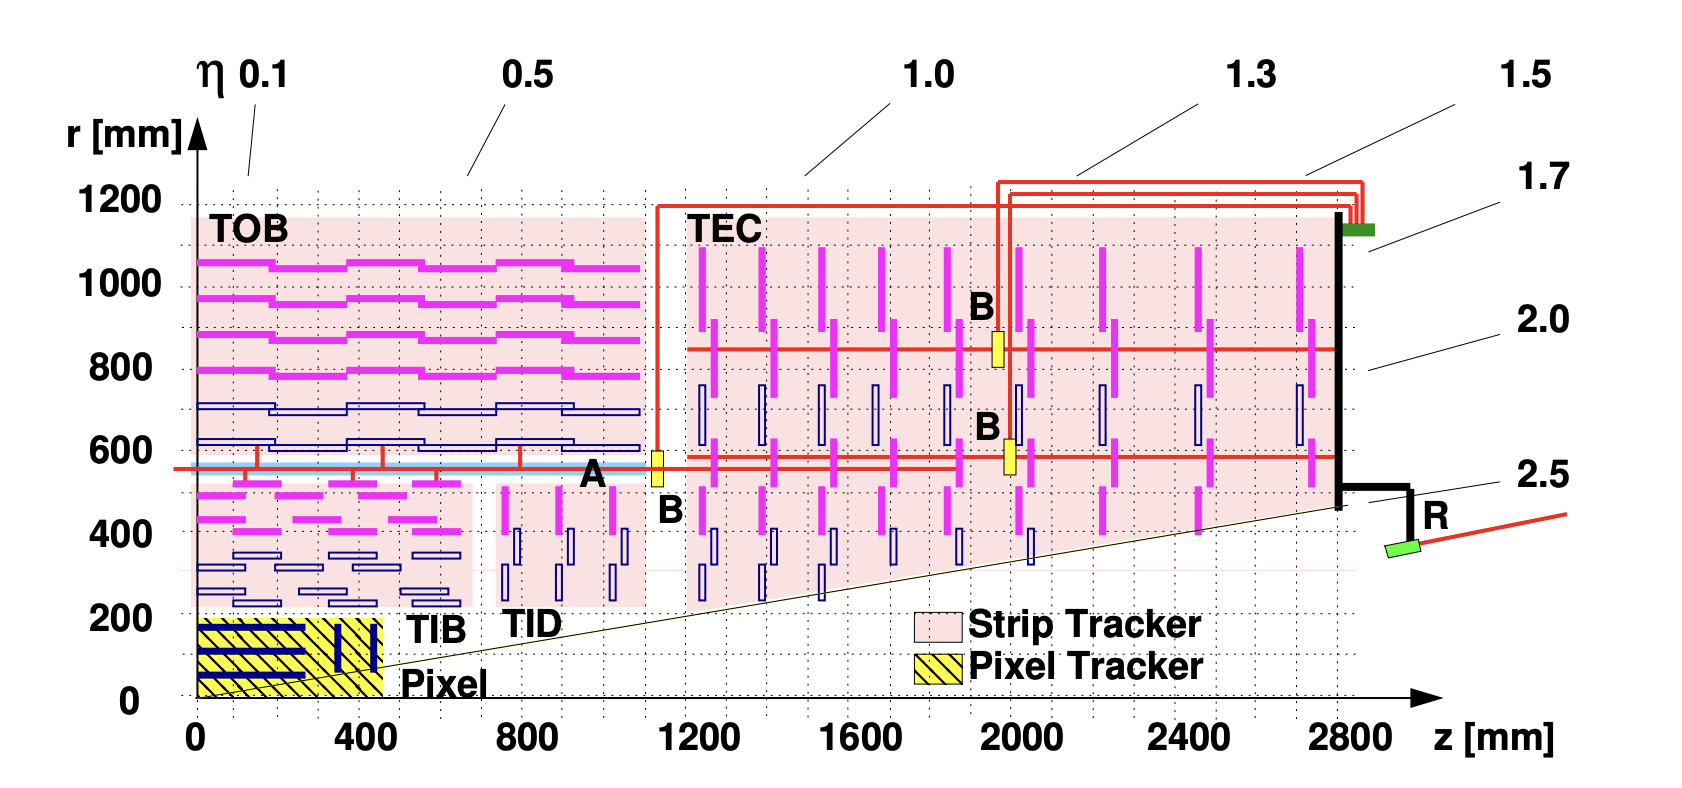
\includegraphics[width=0.8\textwidth]{figures/Part2/CMS/Tracker}
 \end{tabular}
 \caption{A sketch of a quarter of the \ac{CMS} tracker in the $r-z$ plane, adapted from~\cite{CMS:2009dvy}. The strip tracker is shown in pink color, and it is divided into severl parts: the Tracker Inner Barrel (TIB), Tracker Outer Barrel (TOB), Tracker Inner Barrel (TIB), and Tracker Inner Disk (TID). The original pixel detector with three barrel layers is shown in yellow and black colors.}
 \label{fig:Tracker}
 \end{center}
\end{figure}


It uses silicon Pixels and Microstrips to reconstruct the trajectories of charged particles such as electrons and muons, which are then used to determine the momentum as well as the spatial coordinate of these final state particles.

\begin{figure}[tbh!]
 \begin{center}
 \begin{tabular}{c}
 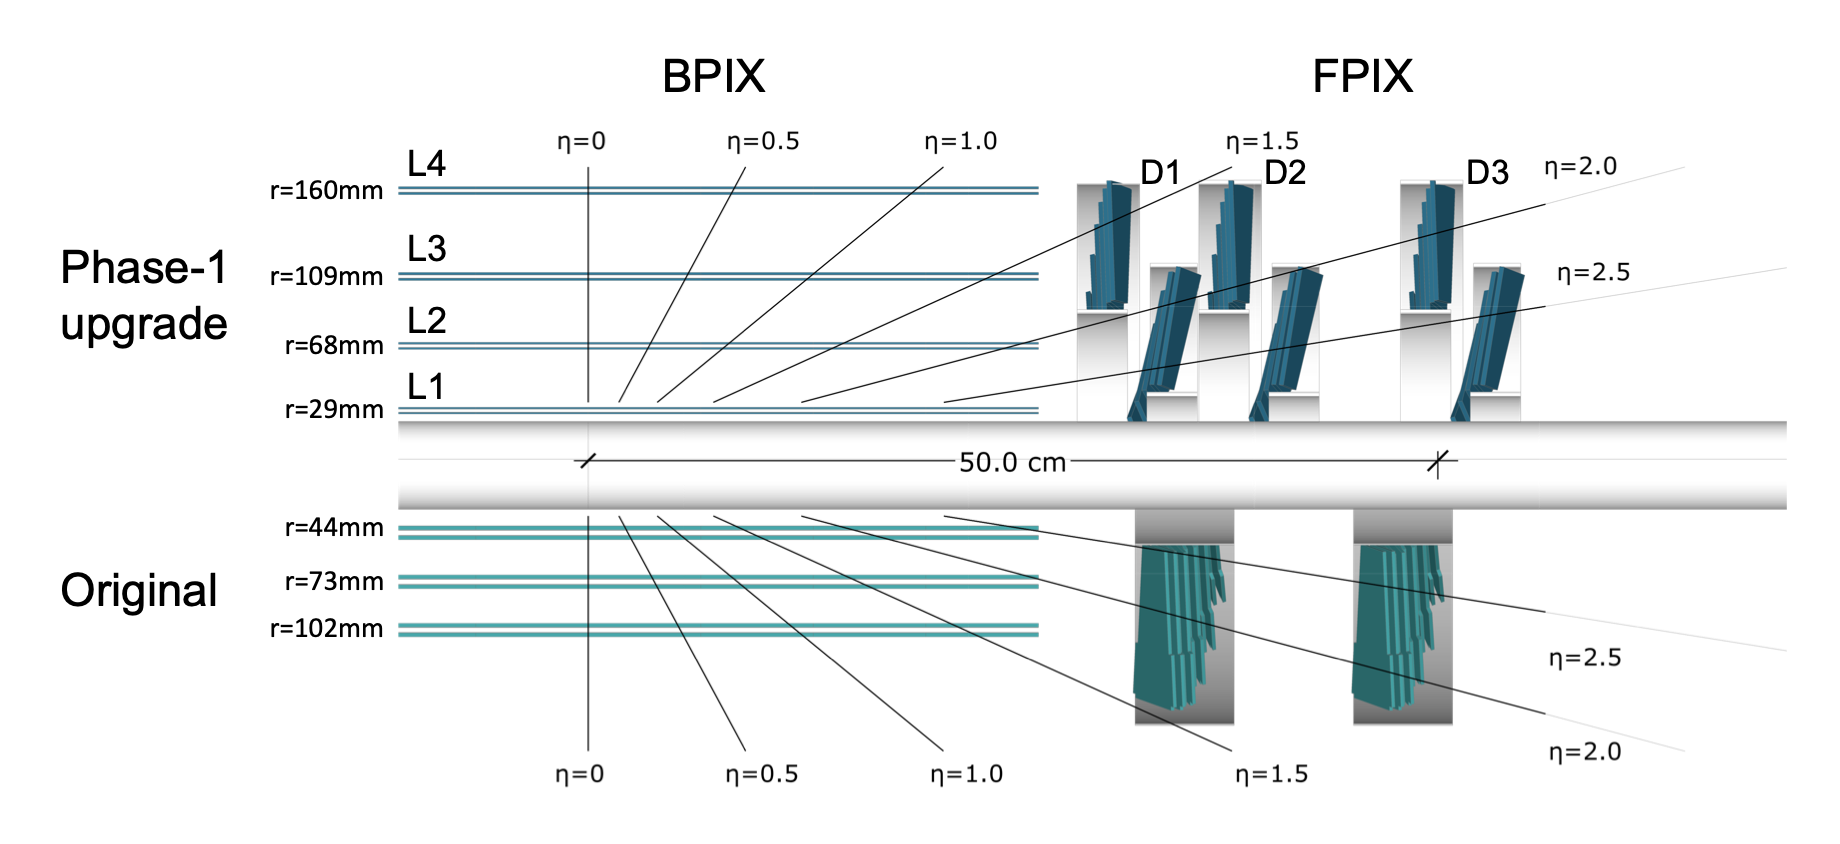
\includegraphics[width=0.8\textwidth]{figures/Part2/CMS/Pixel}
 \end{tabular}
 \caption{A comparison between the original pixel detector and the upgraded pixel detector in the $r-z$ plane, adapted from~\cite{CMSTrackerGroup:2020edz}.}
 \label{fig:Pixel}
 \end{center}
\end{figure}


\section{The Electromagnetic Calorimeter}
\label{sec:ECAL}

The \ac{ECAL} is made of lead tungstate crystals. These dense crystals stop electrons and photons completely and convert their energy into the form of light. The energy of particles can be measured from the intensity of the light.

\section{The Hadronic Calorimeter}
\label{sec:HCAL}

The \ac{HCAL} consists of multiple layers of tiles that form a closed space to ensure high efficiency of missing transverse energy measurement of invisible particles. The tiles stop hadrons completely and transfer the signals to reconstruct the energy and positions of particles.

\section{The Superconducting Magnet}
\label{sec:Magnet}

The superconducting solenoid produces a magnetic field that is close to 4T. The paths of charged particles are curved by this magnetic field in order to identify the charge and momentum of particles. A strong magnetic field is able to curve particles with high energy and provides a good resolution in the high transverse momentum region.

\section{The Muon System}
\label{sec:MuonSys}

The muon detector is the outermost detector of the CMS. The \ac{DT} and \ac{RPC} together make up the barrel region of the muon system, and the end-cap muon system consists of \ac{RPC} and  \ac{CSC}. The \ac{GEM} is the latest addition to the muon system. It complements \ac{CSC} in the forward region. The muon system reconstructs the tracks of muons, and with the strong magnetic field produced by the superconducting solenoid and its iron flux return, the tracks are bent in order to calculate the momentum of muons.

\section{The Trigger System}
\label{sec:TrigSys}

\ac{L1} \ac{HLT} 